% Chapter Template

\chapter{The CUDA Model} % Main chapter title

\label{Chapter2} % Change X to a consecutive number; for referencing this chapter elsewhere, use \ref{ChapterX}

\lhead{Chapter 2. \emph{The CUDA Model}} % Change X to a consecutive number; this is for the header on each page - perhaps a shortened title

%----------------------------------------------------------------------------------------
%	SECTION 1
%----------------------------------------------------------------------------------------

\section{Introduction}


CUDA is a parallel computing platform and programming model that serves as an extension to the C language. It allows development of applications for various kinds of devices, such as personal computers, embedded systems to HPC clustered systems.

In addition to sharing many abstractions with other parallel programming models, the CUDA programming model provides the following special features to harness the computing power of GPU architectures: 
\begin{itemize}
    \item A way to organize threads on the GPU through a hierarchy structure
    \item A way to access memory on the GPU through a hierarchy structure
\end{itemize}

Unlike C parallel programming, where the programmer is responsible for managing threads explicitly using either pthreads or OpenMP techniques, CUDA exposes a thread hierarchy abstraction which allows the programmer to control thread behavior.

\section{CUDA Programming Structure}

The CUDA programming model executes applications on a heterogeneous computing system, which comprises of two distinct program entitites:
\begin{itemize}
	\item \textbf{the host} - the CPU, and its memory (host memory)
	\item \textbf{the device} - The GPU, and its memory (device memory)
\end{itemize}


At the core of the CUDA programming model is the \textbf{kernel} - the code that runs on the GPU hardware. The CUDA model allows developers the freedom to write kernel as a sequential program - abstracting away the parallelism, and manages scheduling the developer-written code on the GPU threads. On the other hand, the host defines the mapping of the algorithm to the device based on parameters such as the application data and the GPU device capability. This model allows developers the benefit of focusing on the algorithm in a scalar fashion, by writing sequential code, and not get distracted by the details and nuances that often come up with creating and managing thousands of GPU threads.


Unless explicitly programmed by the programmer, the host operates independently of the device. When a kernel is launched by the host, the control returns to the host immediately, freeing the CPU to perform additional tasks while the kernel gets executed on the device. The CUDA programming model is asynchronous so the GPU computation happening on the GPU can be overlapped with the host-device communication.  A typical CUDA program consists of the serial host code complemented by the parallel code executing on the device. 

For every computational kernel, the single-threaded host program leverages command queues supported by the OpenCL API to issue commands for  performing the following operations: 

The processing flow in a standard CUDA program follows this sequence:
\begin{itemize}
	\item \textbf{Host to Device or H2D transfer} - copying the data from host to input buffers resident on device memory. 
	\item \textbf{Execution} - launching the kernel in a SIMD fashion on the target device.
	\item \textbf{Device to Host or D2H transfer} - copying back the data stored in output buffers in the device after the kernel has finished processing back to the host memory.
\end{itemize}

As the CUDA programming model assumes a system comprising of a host and a device, each with its separate memory, the model provides functions to allocate and release device memory. In addition, it also provides functions to transfer data between the host and the device memory. This directly follows the processing flow given in the preceding paragraph. The control over both device and host memory is especially important given that the kernels operate out of device memory, and therefore providing complete control over device memory management allows programmers to achieve the best performance.

Another interesting characteristic of the CUDA programming model is the exposed memory hierarchy. Each GPU device has different types of memory used for different purposes. The two main types of memories in any GPU device are the global and the shared memory. The global memory is analogous to the CPU system memory, while the shared memory is similar to the CPU cache. However, and perhaps quite notably, GPU shared memory can be directly controlled from a CUDA kernel.


\begin{figure}[ht]
	\centering
	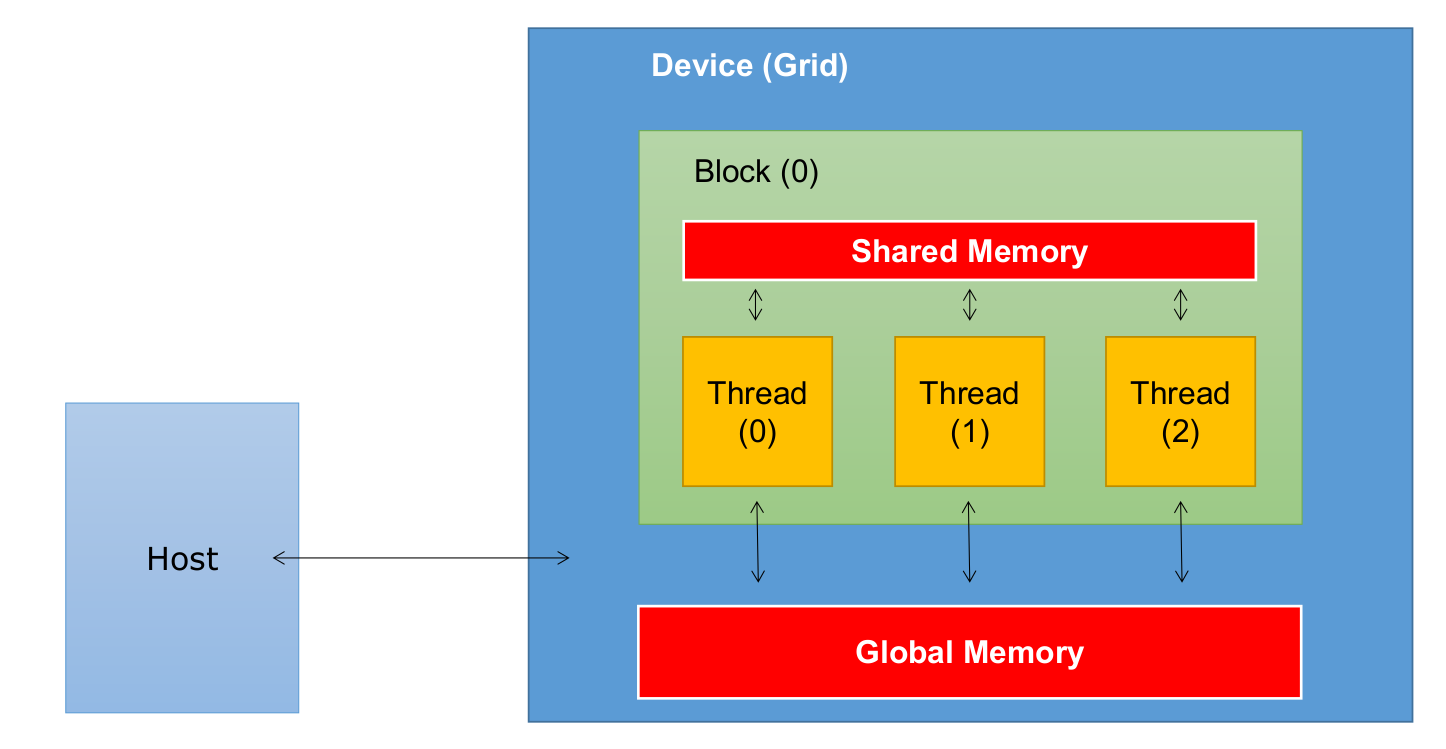
\includegraphics[scale=0.30]{Pictures/ch2/cuda_mem_hierarchy.png}
	\caption{\small CUDA memory hierarchy}
\end{figure}


% thread hierarchy
So far, we have discussed about the memory hierarchy in CUDA and how the different kinds of memory interact with the threads during the execution. The threads in CUDA themselves are organized in a two-tier hierarchy, which can be decomposed into 'blocks' of threads, and 'grids' of blocks.

Whenever a host program launches a kernel with a set number of threads, all threads belong to a single unit called the grid. All threads in a grid share the same global memory space as shown in figure 2.1. Each grid itself comprises of single (or multiple) blocks. A thread block is a localised group of threads which have more intimate cooperation with each other as they interact with each other using:

\begin{itemize}
    \item block-local synchronization
    \item block-local shared memory
\end{itemize}

Threads belonging to different blocks cannot cooperate. 
In order to navigate through this hierarchy and address each thread uniquely, CUDA employs two unique coordinates to distinguish threads:

\begin{itemize}
    \item \textbf{blockIdx}: block index within a grid
    \item \textbf{threadIdx}: thread index within a block
\end{itemize}

These variables are built-in and pre-initialized that can be directly accessed within a kernel. During the kernel execution, the coordinate variables are assigned to each thread automatically by the CUDA runtime. By assigning conditions on the values of these variables, portions of data can be assigned to different threads.

The coordinate variable is of type \textit{uint3}, a CUDA built-in vector type, derived from the basic integer type. It is a structure containing three unsigned integers, and the 1st, 2nd, and 3rd components are accessible through the fields x, y, and z respectively:

% \usepackage{minted}

% \begin{document}
% \begin{minted}{python}
\textit{threadIdx.x    blockIdx.x} \newline
\textit{threadIdx.y    blockIdx.y} \newline
\textit{threadIdx.z    blockIdx.z}

\begin{figure}[ht]
	\centering
	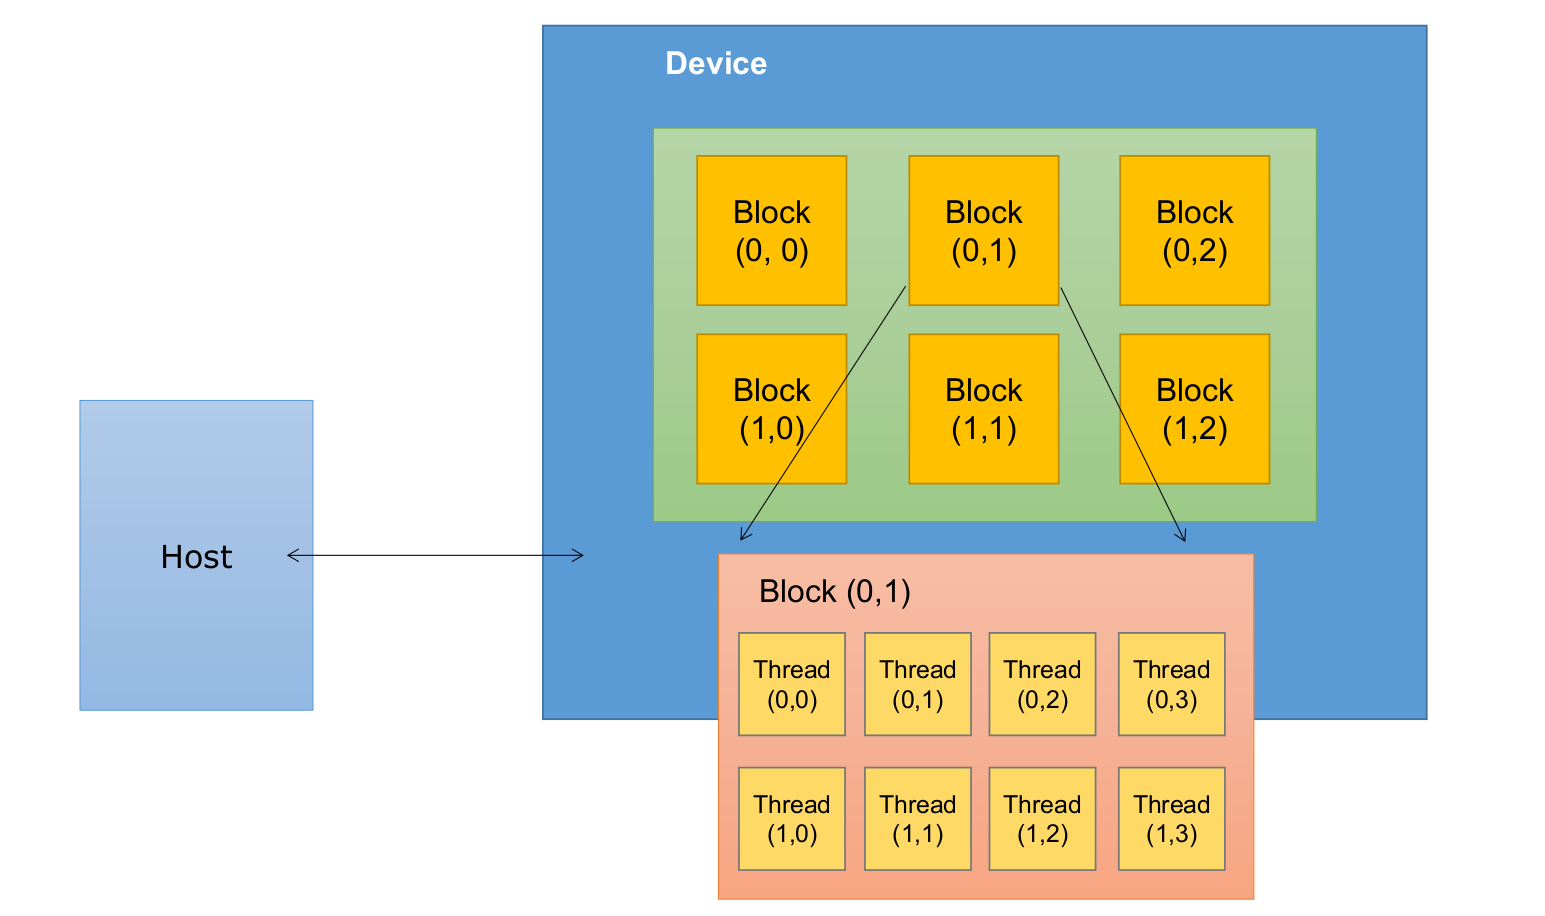
\includegraphics[scale=0.30]{Pictures/ch2/cuda_thread_hierarchy.png}
	\caption{\small CUDA thread hierarchy}
\end{figure}

% threadIdx.x blockIdx.x \newline
% threadIdx.y blockIdx.y
% \end{minted}
% \end{document}

\section{An Example}

	\par As an illustrative example, we consider a simple CUDA application which performs a vector addition. The vector addition kernel $vadd$ executes on device $GPU_0$. It takes as input two input buffers ($in1$ and $in2$) performs element-wise addition and produces an output buffer ($out$). In Fig. \ref{fig:OpenCLArch}, the CUDA host program sets prepares for kernel execution by transfering the input data from the host memory to the device memory through the cudaMemcpy(..cudaMemcpyHostToDevice) instruction. Once the input buffers have been transferred to the device memory, the kernel $addVectors$ is launched with some block and grid dimensions. The mapping is done such that each thread in a thread block would compute exactly one element in the output vector. It is possible, however, that the final block might have some threads which do not map to any element in the output vector (due to block size not being a factor of size of vectors). In this case, threads which are not necessary are disabled through a preliminary if condition in the kernel code.
	
	The kernel code simply calculates the unique global ID of each thread, and computes the corresponding output element with the index equal to the global ID of the thread. The expression $int id = blockIdx.x * blockDim.x + threadIdx.x$ calculates the index of the current thread in the entire grid, which allows us to uniquely identify this thread within the entire grid, and not just the block through a single number.
	
	The kernel execution is completed when all thread blocks finish execution. At this point, the resulting vector $out$ is ready to be copied from the device memory back to the host memory. This is again done using the cudaMemcpy() function except this time we use the cudaMemcpyDeviceToHost object to signal that data is being transferred from device to host this time.
	
	\begin{figure}[ht]  
		\centering
		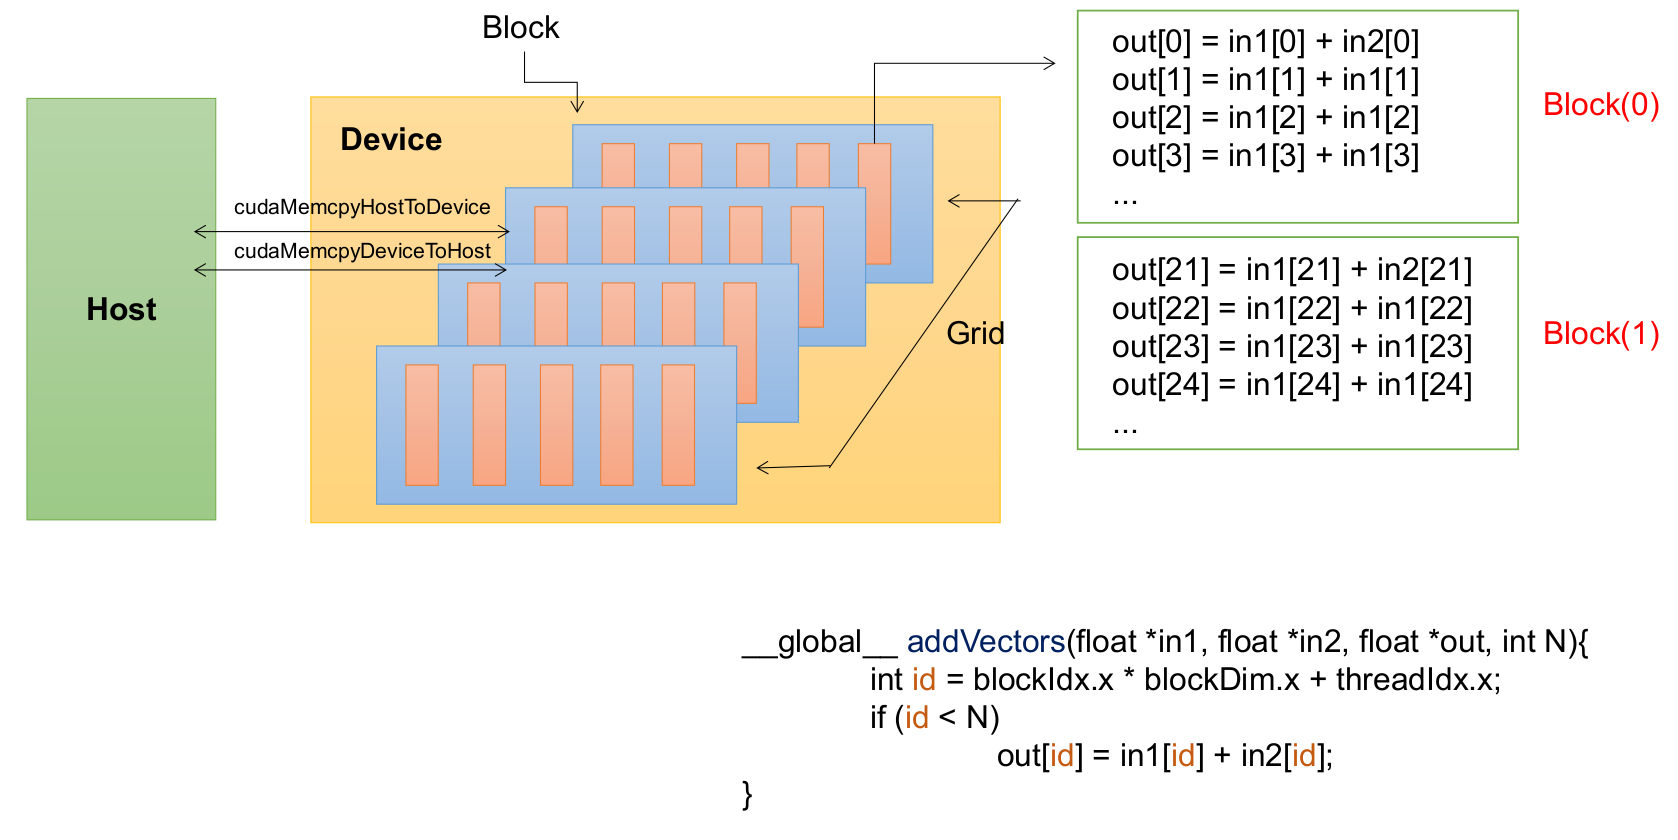
\includegraphics[scale=0.25]{Pictures/ch2/add_example.png}
		\caption{OpenCL Execution \label{fig:OpenCLArch}}
	\end{figure}
	
	However, as explained previously, the host and device are asynchronous, and the control returns back to the host program as soon as the kernel is launched on the device. Therefore, if there is no barrier in place, the control reaches the cudaMemcpy instruction immediately. This might result in incorrect data being copied from the device to host as there is a chance that the kernel execution has not yet finished. This issue was identified by the CUDA developers early on, and therefore, the cudaMemcpy function was thus converted into one of the few synchronous functions in the CUDA library. This ensured that the copy instruction was not executed before the device finished executing the kernel.